\documentclass[10pt,a4paper]{article}
\usepackage[utf8]{inputenc}
\usepackage[T1]{fontenc}
\usepackage{lmodern}
\usepackage[a4paper,margin=1.9cm,top=1.6cm,bottom=1.8cm]{geometry}
\usepackage{microtype}
\usepackage{booktabs,tabularx,array}
\usepackage{enumitem}
\usepackage{xcolor}
\usepackage{tikz}
\usetikzlibrary{automata,positioning,arrows.meta}
\usepackage{titlesec}
\titlespacing*{\section}{0pt}{8pt}{3pt}
\titlespacing*{\subsection}{0pt}{5pt}{2pt}
\titleformat{\section}{\large\bfseries}{\thesection}{0.6em}{}
\titleformat{\subsection}{\normalsize\bfseries}{\thesubsection}{0.6em}{}
\setlength{\parindent}{0pt}
\setlength{\parskip}{3pt}
\setlist{nosep,leftmargin=1.2em}
\newcommand{\tk}[1]{\texttt{#1}}
\renewcommand{\arraystretch}{1.12}

\begin{document}

\begin{center}
{\small UTAD \textbar\ Licenciatura em Engenharia Informática \textbar\ Compiladores}\\[3pt]
{\Large\bfseries Trabalho Prático 1 -- Análise lexical da linguagem GreenScript}\\[5pt]
\begin{tabular}{ll}
{[Nome do estudante 1]} & n.º {[número 1]}\\
{[Nome do estudante 2]} & n.º {[número 2]}\\
{[Nome do estudante 3]} & n.º {[número 3]}
\end{tabular}
\end{center}

\section{Objetivo e abordagem}
Foi implementado em FLEX o analisador lexical da linguagem GreenScript. O programa lê o ficheiro cujo caminho
recebe como argumento e escreve, pela ordem de ocorrência, uma linha por token no formato
\tk{linha CATEGORIA lexema}. Os erros lexicais aparecem no mesmo fluxo, na posição em que ocorrem, como
\tk{linha ERRO\_LEXICO lexema (motivo)}. No fim é apresentado o resumo \tk{Tokens: N | Erros lexicais: M}.
O analisador não verifica a ordem dos tokens, o número de argumentos nem a correspondência de parênteses e chavetas,
que ficam para a análise sintática (TP2).

A decisão central é a \emph{regra do candidato lexical}: qualquer sequência máxima de letras ASCII, algarismos,
\tk{-} ou \tk{\_} é tratada como uma unidade. O FLEX escolhe sempre a correspondência mais longa e, em caso de empate,
a regra escrita primeiro. Por isso basta colocar as palavras reservadas, o identificador de estufa e o inteiro
\emph{antes} de uma regra genérica \tk{[A-Za-z0-9\_-]+}. Se a sequência for exatamente uma palavra reservada,
um identificador ou um inteiro, há empate de comprimento e vence a regra específica. Se for mais longa (\tk{LIGARX},
\tk{12abc}, \tk{EST-AA001}), vence a regra genérica e é emitido um único erro para a sequência inteira, sem tokens parciais.

\section{Expressões regulares}
\begin{tabularx}{\textwidth}{@{}l>{\raggedright\arraybackslash}p{4.9cm}>{\raggedright\arraybackslash}X@{}}
\toprule
\textbf{Categoria} & \textbf{Expressão regular (FLEX)} & \textbf{Exemplos válidos / inválidos}\\
\midrule
Palavras reservadas & \tk{LIGAR|DESLIGAR|ABRIR|} \tk{FECHAR|AQUECER|PARAR|} \tk{REGAR|ESPERAR|SE|} \tk{SENAO|HUMIDADE|REPETIR} (uma regra por palavra) &
  \tk{LIGAR}, \tk{SENAO} \,/\, \tk{ligar}, \tk{Ligar}, \tk{LIGARX}, \tk{DESLIGAR\_}\\
Identificador de estufa & \tk{EST-[A-Z]\{2\}[0-9]\{2\}} & \tk{EST-AB07}, \tk{EST-ZZ99} \,/\, \tk{EST-AA001}, \tk{EST-A101}, \tk{EST-aa01}, \tk{EST\_AA01}\\
Inteiro & \tk{0|[1-9][0-9]*} & \tk{0}, \tk{15}, \tk{100} \,/\, \tk{012}, \tk{00}, \tk{12abc}, \tk{-5}, \tk{1.5}\\
Candidato inválido & \tk{[A-Za-z0-9\_-]+} (depois das anteriores) & sequências que não são exatamente uma das três categorias acima\\
Delimitadores & \tk{"(" ")" "\{" "\}" "," ";"} & \tk{(}, \tk{\}}, \tk{;} \,/\, \tk{[}, \tk{]}\\
Operadores relacionais & \tk{"<=" ">=" "==" "!=" "<" ">"} & \tk{<=}, \tk{!=} \,/\, \tk{=} e \tk{!} isolados; \tk{<==} dá \tk{<=} e erro em \tk{=}\\
Mudança de linha & \tk{\textbackslash r\textbackslash n|\textbackslash n} & LF e CRLF contam como uma só linha\\
Espaços & \tk{[ \textbackslash t\textbackslash r]+} & ignorados (inclui um CR isolado)\\
Comentário & \tk{"\#"[\textasciicircum\textbackslash n]*} & \tk{\# Preparação da estufa} (UTF-8 aceite)\\
Não reconhecido & \tk{[\textbackslash xC2-\textbackslash xF4][\textbackslash x80-\textbackslash xBF]+} e \tk{.} & \tk{@}, \tk{+}, \tk{*}, \tk{\&}, \tk{ç} (um erro por carácter)\\
\bottomrule
\end{tabularx}

O comentário consome tudo até ao \tk{\textbackslash n} sem o incluir, pelo que a mudança de linha continua a ser contada,
e funciona também quando o ficheiro termina sem mudança de linha. Como o comentário é a correspondência mais longa
a partir de \tk{\#}, nenhum conteúdo no seu interior (incluindo \tk{@}, \tk{=} ou UTF-8) gera tokens ou erros.
A regra \tk{UTF8\_MULTI} agrupa os bytes de um carácter UTF-8 multibyte fora de comentários, para que \tk{ç} gere um
só erro e não dois.

\section{Autómato finito determinístico do identificador de estufa}
O AFD $A = (Q, \Sigma, \delta, q_0, F)$ reconhece exatamente a linguagem \tk{EST-[A-Z]\{2\}[0-9]\{2\}}:
\begin{itemize}
\item $\Sigma$: caracteres ASCII; nas transições usam-se as classes $M = \{A,\dots,Z\}$ (maiúsculas) e $D = \{0,\dots,9\}$ (algarismos).
\item $Q = \{q_0,\dots,q_8, q_R\}$; estado inicial $q_0$; estados finais $F = \{q_8\}$; $q_R$ é o estado de rejeição (sumidouro).
\item Qualquer símbolo sem transição indicada leva a $q_R$, incluindo qualquer símbolo lido em $q_8$. Por isso
\tk{EST-AA001} e \tk{EST-AA01X} são rejeitados. De $q_R$ não se sai.
\end{itemize}

\begin{center}
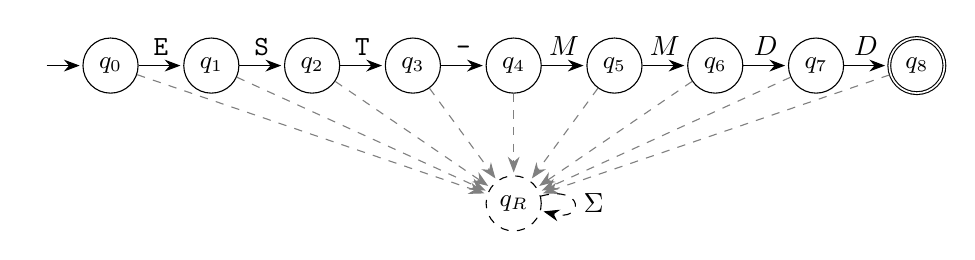
\begin{tikzpicture}[shorten >=1pt, node distance=1.28cm, on grid, auto, >={Stealth[length=2mm]},
  every state/.style={minimum size=7mm, inner sep=0pt, font=\small}]
  \node[state, initial, initial text={}] (q0) {$q_0$};
  \node[state] (q1) [right=of q0] {$q_1$};
  \node[state] (q2) [right=of q1] {$q_2$};
  \node[state] (q3) [right=of q2] {$q_3$};
  \node[state] (q4) [right=of q3] {$q_4$};
  \node[state] (q5) [right=of q4] {$q_5$};
  \node[state] (q6) [right=of q5] {$q_6$};
  \node[state] (q7) [right=of q6] {$q_7$};
  \node[state, accepting] (q8) [right=of q7] {$q_8$};
  \node[state, dashed] (qR) [below=1.75cm of q4] {$q_R$};
  \path[->] (q0) edge node {\tk{E}} (q1)
            (q1) edge node {\tk{S}} (q2)
            (q2) edge node {\tk{T}} (q3)
            (q3) edge node {\tk{-}} (q4)
            (q4) edge node {$M$} (q5)
            (q5) edge node {$M$} (q6)
            (q6) edge node {$D$} (q7)
            (q7) edge node {$D$} (q8);
  \foreach \s in {q0,q1,q2,q3,q4,q5,q6,q7,q8}
     \path[->, dashed, gray] (\s) edge (qR);
  \path[->, dashed] (qR) edge [loop right] node {$\Sigma$} ();
\end{tikzpicture}\\[1pt]
{\small Setas a tracejado: todos os restantes símbolos de $\Sigma$ (outro).}
\end{center}

\begin{center}\small
\begin{tabular}{@{}l*{8}{c}c@{}}
\toprule
$\delta$ & \tk{E} & \tk{S} & \tk{T} & \tk{-} & $M\setminus\{E,S,T\}$ & $D$ & outro\\
\midrule
$\to q_0$ & $q_1$ & $q_R$ & $q_R$ & $q_R$ & $q_R$ & $q_R$ & $q_R$\\
$q_1$ & $q_R$ & $q_2$ & $q_R$ & $q_R$ & $q_R$ & $q_R$ & $q_R$\\
$q_2$ & $q_R$ & $q_R$ & $q_3$ & $q_R$ & $q_R$ & $q_R$ & $q_R$\\
$q_3$ & $q_R$ & $q_R$ & $q_R$ & $q_4$ & $q_R$ & $q_R$ & $q_R$\\
$q_4$ & $q_5$ & $q_5$ & $q_5$ & $q_R$ & $q_5$ & $q_R$ & $q_R$\\
$q_5$ & $q_6$ & $q_6$ & $q_6$ & $q_R$ & $q_6$ & $q_R$ & $q_R$\\
$q_6$ & $q_R$ & $q_R$ & $q_R$ & $q_R$ & $q_R$ & $q_7$ & $q_R$\\
$q_7$ & $q_R$ & $q_R$ & $q_R$ & $q_R$ & $q_R$ & $q_8$ & $q_R$\\
$*q_8$ & $q_R$ & $q_R$ & $q_R$ & $q_R$ & $q_R$ & $q_R$ & $q_R$\\
$q_R$ & $q_R$ & $q_R$ & $q_R$ & $q_R$ & $q_R$ & $q_R$ & $q_R$\\
\bottomrule
\end{tabular}
\end{center}
Exemplos: \tk{EST-AB07} percorre $q_0 q_1 q_2 q_3 q_4 q_5 q_6 q_7 q_8$ e é aceite. Em \tk{EST-A101}, o \tk{1}
lido em $q_5$ leva a $q_R$. Em \tk{EST-aa01}, o \tk{a} lido em $q_4$ leva a $q_R$. \tk{EST-AA1} termina em $q_7$, que não é final.

\section{Implementação em FLEX}
\begin{itemize}
\item \textbf{Ficheiro} \tk{src/greenscript.l}, com as opções \tk{noyywrap}, \tk{nounput} e \tk{noinput}. A função \tk{main} abre
\tk{argv[1]} em \tk{yyin}, em modo binário para preservar o CR, chama \tk{yylex()} e imprime os totais. Devolve 0 sem
erros, 1 com erros lexicais e 2 em erro de utilização.
\item \textbf{Ordem das regras:} separadores e comentários; as 12 palavras reservadas; \tk{ID\_ESTUFA}; \tk{INTEIRO}; o
candidato genérico; os operadores de dois caracteres antes dos de um; os delimitadores; e, por fim, \tk{=}, \tk{!},
UTF-8 multibyte e \tk{.} como erros. A correspondência mais longa garante que \tk{<=}, \tk{>=}, \tk{==} e \tk{!=} nunca
são divididos.
\item \textbf{Linhas:} o contador \tk{linha} começa em 1 e é incrementado apenas pela regra \tk{\textbackslash r\textbackslash n|\textbackslash n}.
Nenhum token contém mudanças de linha, por isso a linha registada é a linha de início do token.
\item \textbf{Erros e continuação:} as funções \tk{token()} e \tk{erro()} escrevem a linha e o lexema e atualizam os contadores.
Depois de um erro, o FLEX continua no carácter seguinte ao lexema consumido, que é o candidato completo ou o carácter
isolado. Para diagnósticos mais claros, um candidato inválido é classificado como
\emph{identificador de estufa malformado} (começa por \tk{EST-}), \emph{inteiro malformado} (começa por algarismo)
ou \emph{sequência inválida}.
\item \textbf{Categorias:} o nome da palavra reservada (\tk{LIGAR}, \dots, \tk{REPETIR}), \tk{ID\_ESTUFA}, \tk{INTEIRO},
\tk{ABRE\_PAR}, \tk{FECHA\_PAR}, \tk{ABRE\_CHAVETA}, \tk{FECHA\_CHAVETA}, \tk{VIRGULA}, \tk{PONTO\_VIRG}, \tk{MENOR},
\tk{MENOR\_IGUAL}, \tk{MAIOR}, \tk{MAIOR\_IGUAL}, \tk{IGUAL}, \tk{DIFERENTE} e \tk{ERRO\_LEXICO}. Os inteiros são
guardados como texto, sem conversão numérica.
\end{itemize}

\section{Testes}
\sloppy Cada ficheiro \tk{testes/NN\_nome.gs} tem o resultado esperado em \tk{NN\_nome.esperado}. O script
\tk{testes/correr\_testes.sh} (ou \tk{make testes}) executa todos os testes e compara as saídas com \tk{diff}.
Os 10 testes passam.

\begin{center}\small
\begin{tabularx}{\textwidth}{@{}l>{\raggedright\arraybackslash}Xrr@{}}
\toprule
\textbf{Teste} & \textbf{Conteúdo} & \textbf{Tokens} & \textbf{Erros}\\
\midrule
01\_comandos\_simples & todos os comandos, \tk{EST-AA01}, \tk{0} e \tk{100} & 45 & 0\\
02\_espera\_repetir & \tk{ESPERAR}, \tk{REPETIR(3)\{\dots\}} e \tk{REPETIR} contendo \tk{SE}/\tk{SENAO}, tabulação, linhas vazias & 69 & 0\\
03\_condicao\_operadores & \tk{SE}/\tk{SENAO} com os 6 operadores, com e sem espaços (\tk{HUMIDADE(2)<=30}) & 141 & 0\\
04\_sintaxe\_incorreta & \tk{LIGAR();}, \tk{REGAR(1);}, \tk{) ( \} \{}, \tk{FECHAR(EST-QW12,,,);}: válidos lexicalmente & 35 & 0\\
05\_erros\_candidatos & \tk{LIGARX}, \tk{ligar}, \tk{EST-AA001}, \tk{EST-A101}, \tk{012}, \tk{12abc}, \tk{REGAR(2,015);} \dots & 12 & 19\\
06\_erros\_caracteres & \tk{@}, \tk{=} e \tk{!} isolados, \tk{<==}, \tk{=!}, \tk{+}, \tk{*}, \tk{1.5}, \tk{-5}, \tk{ç} \dots & 55 & 23\\
07\_comentarios\_separadores & só comentários (com UTF-8 e \tk{@ = !}), espaços, CRLF, sem \tk{\textbackslash n} final & 0 & 0\\
08\_vazio & ficheiro vazio & 0 & 0\\
09\_exemplo\_enunciado & exemplo da secção 5 do enunciado & 12 & 0\\
10\_crlf\_fim\_ficheiro & terminações CRLF e fim de ficheiro sem mudança de linha & 13 & 0\\
\bottomrule
\end{tabularx}
\end{center}

Excerto da saída do teste 06 (linha \tk{HUMIDADE(2)<==30}), que mostra a correspondência mais longa e a continuação após o erro:\\
\tk{5 MENOR\_IGUAL <=}\quad \tk{5 ERRO\_LEXICO = ('=' isolado nao e operador)}\quad \tk{5 INTEIRO 30}

\section{Ferramentas e fontes}
GNU Flex 2.6.4, GCC e GNU Make em Linux. Relatório em \LaTeX{} (TikZ para o AFD). Não foram usadas bibliotecas além
da biblioteca padrão de C. Referências: enunciado do TP1 e manual do GNU Flex (\emph{Lexical Analysis With Flex}).
Ferramenta de apoio: [indicar aqui se foi usado assistente de IA, conforme as regras da unidade curricular].

\end{document}
